%!TEX program = xelatex
\documentclass[UTF8]{ctexart}
\usepackage{ctex}

\usepackage{geometry}% 版面大小
\geometry{a4paper,scale=0.7}

\usepackage{graphicx}
\graphicspath{{assets/}}
\usepackage{caption2}
\usepackage{subfigure}
\usepackage{float}

\usepackage[hidelinks]{hyperref}

\usepackage{listings}
\usepackage{xcolor}      %代码着色宏包
\usepackage{CJK}         %显示中文宏包


\definecolor{mGreen}{rgb}{0,0.6,0}
\definecolor{mGray}{rgb}{0.5,0.5,0.5}
\definecolor{mPurple}{rgb}{0.58,0,0.82}
\definecolor{backgroundColour}{rgb}{0.95,0.95,0.92}

\lstdefinestyle{CStyle}{
    backgroundcolor=\color{backgroundColour},
    commentstyle=\color{mGreen},
    keywordstyle=\color{magenta},
    numberstyle=\tiny\color{mGray},
    stringstyle=\color{mPurple},
    basicstyle=\footnotesize,
    breakatwhitespace=false,
    breaklines=true,
    captionpos=b,
    keepspaces=true,
    numbers=left,
    numbersep=5pt,
    showspaces=false,
    showstringspaces=false,
    showtabs=false,
    tabsize=2,
    language=C
}

% \lstset{language=C}
% \begin{lstlisting}[style=CStyle]
% #include <stdio.h>
% int main(void)
% {
%    printf("Hello World!"); 
% }
% \end{lstlisting}

\title{\textbf{PA1 实验报告}}
\author{刘时宜 201180078}
\date{\today}

\begin{document}
\maketitle
\tableofcontents

\section{PA1-1}
参考实验说明,在\verb|nemu/include/cpu/reg.h|中修改\verb|CPU_STATE|的定义即可,其中将一些原有代码中的\verb|struct|关键字改成了\verb|union|关键字。修改如下(与实验说明中相同):

\lstset{language=C}
\begin{lstlisting}[style=CStyle]
typedef struct 
{
    union {
        union {
            union {
                uint32_t _32;
                uint16_t _16;
                uint8_t _8[2];
            };
            uint32_t val;
        } gpr[8];
        struct { // do not change the order of the registers
            uint32_t eax, ecx, edx, ebx, esp, ebp, esi, edi;
        };
    };
} CPU_STATE;
\end{lstlisting}

修改后在\verb|~/pa_nju|目录下执行\verb|make clean|、\verb|make|编译项目,然后\verb|make test_pa-1|执行测试用例,可以看到\verb|reg_test()  pass|的提示,说明CPU寄存器模拟成功

\subsection{思考题}
\paragraph{C语言中的struct和union关键字都是什么含义,寄存器结构体的参考实现为什么把部分struct改成了union?}~
\par \verb|struct|关键字在中文中的翻译为“结构体”,\verb|union|关键字在中文中的翻译为“联合体”。两者都是c语言中复杂数据结构类型的实现方式。不同点在于,\verb|struct|中定义的各基本数据占用的是不同的内存空间,不同数据互不干扰。而\verb|union|中定义的各基本数据占用的是相同的内存空间,数据最低位对齐,整个\verb|union|数据结构所占内存空间与其中占内存最大的数据所用的内存相同。
\par 由CPU中寄存器的定义方式,例如\verb|eax|寄存器的低16位称为\verb|ax|,\verb|ax|的低8位称为\verb|al|,可知\verb|eax|、\verb|ax|、\verb|al|、\verb|ah|本质上占用的是一块内存空间,相互之间有影响,与\verb|union|中各数据类型相互影响的定义相同,故应该采用\verb|union|关键字进行定义。

\section{PA1-2}
\subsection{add}
参照给出的样例实现代码,填入\verb|alu_add|中。

\lstset{language=C}
\begin{lstlisting}[style=CStyle]
uint32_t alu_add(uint32_t src, uint32_t dest, size_t data_size){
    uint32_t res = 0;
    res = dest + src;
    
    set_CF_add(res, dest, data_size);
    set_PF(res);
    set_ZF(res, data_size);
    set_SF(res, data_size);
    set_OF_add(res, src, dest, data_size);
    
    return res & (0xFFFFFFFF >> (32 - data_size));
    
}
\end{lstlisting}

然后,同样写出其中引用的函数。

\begin{lstlisting}[style=CStyle]
inline void set_ZF(uint32_t result, size_t data_size){
    result = sign_ext(result & (0xFFFFFFFF >> (32 - data_size)), data_size);
    cpu.eflags.ZF = (result == 0);
}

inline void set_SF(uint32_t result, size_t data_size){
    result = sign_ext(result & (0xFFFFFFFF >> (32 - data_size)), data_size);
    cpu.eflags.SF = sign(result);
}

inline void set_PF(uint32_t result){
    int count = 0;
    result = result & (0xFF);
    
    while(result){
        count += result & 0x1;
        result = result >> 1;
    }
    
    cpu.eflags.PF = !(count % 2);
}

inline void set_CF_add(uint32_t result, uint32_t src, size_t data_size){
    result = sign_ext(result & (0xFFFFFFFF >> (32 - data_size)), data_size);
    src = sign_ext(src & (0xFFFFFFFF >> (32 - data_size)), data_size);
    cpu.eflags.CF = result < src;
}

inline void set_OF_add(uint32_t result, uint32_t src, uint32_t dest, size_t data_size){
    switch(data_size){
        case 8:
            result = sign_ext(result & 0xFF, 8);
            src = sign_ext(src & 0xFF, 8);
            dest = sign_ext(dest & 0xFF, 8);
            break;
        case 16:
            result = sign_ext(result & 0xFFFF, 16);
            src = sign_ext(src & 0xFFFF, 16);
            dest = sign_ext(dest & 0xFFFF, 16);
            break;
        default: break;
    }
    
    
    if(sign(src) == sign(dest)){
        if(sign(src) != sign(result))
            cpu.eflags.OF = 1;
        else
            cpu.eflags.OF = 0;
    }
    else{
        cpu.eflags.OF = 0;
    }
}
\end{lstlisting}

\verb|make test_pa-1|后通过了测试样例。

\subsection{adc}
带进位的加法与add中的实现几乎相同,除了判断CF标志位的时候有所改变。原先由于变量大小关系,若有进位结果一定小于原先的操作数。有进位输入之后,产生进位输出时结果也可能等于原先的操作数。因此要根据原先CF位的值做不同判断。

\begin{lstlisting}[style=CStyle]
inline void set_CF_adc(uint32_t result, uint32_t src, uint32_t cf, size_t data_size){
    result = sign_ext(result & (0xFFFFFFFF >> (32 - data_size)), data_size);
    src = sign_ext(src & (0xFFFFFFFF >> (32 - data_size)), data_size);
    if(cf)
        cpu.eflags.CF = result <= src;
    else
        cpu.eflags.CF = result < src;
}

uint32_t alu_adc(uint32_t src, uint32_t dest, size_t data_size){
    // printf("src: %08x, dest: %08x, CF: %01x, data_size: %d\n", src, dest, cpu.eflags.CF, data_size);
    uint32_t res = 0;
    res = dest + src + cpu.eflags.CF;
    // printf("res: %08x\n", res);
    
    set_CF_adc(res, dest, cpu.eflags.CF, data_size);
    set_PF(res);
    set_ZF(res, data_size);
    set_SF(res, data_size);
    set_OF_add(res, src, dest, data_size);
    
    return res & (0xFFFFFFFF >> (32 - data_size));
}
\end{lstlisting}

\subsection{sub}

无借位减法sbb的实现,除了更改运算符号为“-”以外,还要特别处理CF和OF标志位的处理函数。
\par CF标志位设置函数中吧CF值的表达式改为\verb|cpu.eflags.CF = result > dest;|,吧小于号改为大于号即可。
\par OF标志位在将减数取补码的基础上,绝大多数代码沿用add中OF标志位设置函数的代码即可。唯一要注意的一点是机器数全为1的数补码为其自身,此时取补码后简单沿用相加的判定标准会出错。将这部分做特殊情况处理即可,即\verb|invalid complement|相关代码部分。

\begin{lstlisting}[style=CStyle]
inline void set_CF_sub(uint32_t result, uint32_t dest, size_t data_size){
    // printf("In set_CF_sub:\n");
    result = sign_ext(result & (0xFFFFFFFF >> (32 - data_size)), data_size);
    dest = sign_ext(dest & (0xFFFFFFFF >> (32 - data_size)), data_size);
    cpu.eflags.CF = result > dest;
    // printf("    dest: %08x, result: %08x, data_size: %d\n", dest, result, data_size);
    // printf("    CF: %d\n", cpu.eflags.CF);
}

void set_OF_sub(uint32_t result, uint32_t src, uint32_t dest, size_t data_size){
    //printf("In set_OF_sub:\n");
    int invalid_complement = 0;
    switch(data_size){
        case 8:
            result = sign_ext(result & 0xFF, 8);
            src = sign_ext(src & 0xFF, 8);
            dest = sign_ext(dest & 0xFF, 8);
            if(src == 0x80)
                invalid_complement = 1;
            break;
        case 16:
            result = sign_ext(result & 0xFFFF, 16);
            src = sign_ext(src & 0xFFFF, 16);
            dest = sign_ext(dest & 0xFFFF, 16);
            if(src == 0x8000)
                invalid_complement = 1;
            break;
        default: 
            if(src == 0x80000000)
                invalid_complement = 1;
            break;
    }
    //printf("    dest: %08x, result: %08x, data_size: %d\n", dest, result, data_size);
    
    if(invalid_complement){
        if(!sign(dest)){//dest >= 0, certainly overflow
            cpu.eflags.OF = 1;
            //printf("    OF: 1, invalid complement.\n");
            return;
        }
        else{
            cpu.eflags.OF = 0;
            //printf("    OF: 0, invalid complement.\n");
            return;
        }
    }
    
    src = ~src + 1;
    if(sign(src) == sign(dest)){
        if(sign(dest) != sign(result)){
            cpu.eflags.OF = 1;
            //printf("    OF: 1\n");
        }
        else{
            cpu.eflags.OF = 0;
            //printf("    OF: 0\n");
        }
    }
    else{
        cpu.eflags.OF = 0;
        //printf("    OF: 0\n");
    }
}

uint32_t alu_sub(uint32_t src, uint32_t dest, size_t data_size){
    //printf("dest: %08x, src: %08x, data_size: %d\n", dest, src, data_size);
    uint32_t res = 0;
    res = dest - src;
    //printf("res: %08x\n", res);
    
    set_CF_sub(res, dest, data_size);
    set_PF(res);
    set_ZF(res, data_size);
    set_SF(res, data_size);
    set_OF_sub(res, src, dest, data_size);
    
    return res & (0xFFFFFFFF >> (32 - data_size));
}
\end{lstlisting}

\subsection{sbb}
sbb函数中,在sub函数的基础上,额外减去借位即可。需要额外处理的标志位仍然是CF和OF。
\par \verb|set_CF_sbb|函数中,仍然需要根据借位的情况,使用大于或者大于等于的判断标准,与\verb|set_CF_adc|函数中类似。
\par \verb|set_OF_sbb|函数中,除了减数本身的补码表示可能是自身外,还要考虑借位后补码不正常的影响,需要多一些特殊情况的分类与处理。

\begin{lstlisting}[style=CStyle]
inline void set_CF_sbb(uint32_t result, uint32_t dest, uint32_t cf, size_t data_size){
    // printf("In set_CF_sub:\n");
    result = sign_ext(result & (0xFFFFFFFF >> (32 - data_size)), data_size);
    dest = sign_ext(dest & (0xFFFFFFFF >> (32 - data_size)), data_size);
    if(cf)
        cpu.eflags.CF = (result >= dest);
    else
        cpu.eflags.CF = (result > dest);
    // printf("    dest: %08x, result: %08x, data_size: %d\n", dest, result, data_size);
    // printf("    CF: %d\n", cpu.eflags.CF);
}

void set_OF_sbb(uint32_t result, uint32_t src, uint32_t dest, uint32_t cf, size_t data_size){
    //printf("In set_OF_sub:\n");
    int invalid_complement = 0;
    switch(data_size){
        case 8:
            result = sign_ext(result & 0xFF, 8);
            src = sign_ext(src & 0xFF, 8);
            dest = sign_ext(dest & 0xFF, 8);
            if(src == 0x80)
                invalid_complement = 1;
            break;
        case 16:
            result = sign_ext(result & 0xFFFF, 16);
            src = sign_ext(src & 0xFFFF, 16);
            dest = sign_ext(dest & 0xFFFF, 16);
            if(src == 0x8000)
                invalid_complement = 1;
            break;
        default: 
            if(src == 0x80000000)
                invalid_complement = 1;
            break;
    }
    //printf("    dest: %08x, result: %08x, data_size: %d\n", dest, result, data_size);
    
    if(invalid_complement){
        if(!cf){
            if(!sign(dest)){//dest >= 0, certainly overflow
                cpu.eflags.OF = 1;
                //printf("    OF: 1, invalid complement, cf = 0\n");
                return;
            }
            else{
                cpu.eflags.OF = 0;
                //printf("    OF: 0, invalid complement, cf = 0\n");
                return;
            }
        }
        else{
            if(!sign(dest) && (dest != 0)){//dest >= 0, certainly overflow
                cpu.eflags.OF = 1;
                //printf("    OF: 1, invalid complement, cf = 1\n");
                return;
            }
            else{
                cpu.eflags.OF = 0;
                //printf("    OF: 0, invalid complement, cf = 1\n");
                return;
            }
        }
    }
    
    src = ~src + 1 - cf;
    //printf("    dest: %08x, result: %08x, data_size: %d\n", dest, result, data_size);
    if(sign(src) == sign(dest)){
        if(sign(dest) != sign(result)){
            cpu.eflags.OF = 1;
            //printf("    OF: 1\n");
        }
        else{
            cpu.eflags.OF = 0;
            //printf("    OF: 0\n");
        }
    }
    else{
        cpu.eflags.OF = 0;
        //printf("    OF: 0\n");
    }
}

uint32_t alu_sbb(uint32_t src, uint32_t dest, size_t data_size){
    //printf("\ndest: %08x, src: %08x, CF: %d, data_size: %d\n", dest, src, cpu.eflags.CF, data_size);
    uint32_t res = 0;
    res = dest - src - cpu.eflags.CF;
    //printf("res: %08x\n", res);
    
    set_OF_sbb(res, src, dest, cpu.eflags.CF, data_size);
    set_CF_sbb(res, dest, cpu.eflags.CF, data_size);
    set_PF(res);
    set_ZF(res, data_size);
    set_SF(res, data_size);
    
    return res & (0xFFFFFFFF >> (32 - data_size));
}
\end{lstlisting}

\subsection{mul}
将两操作数根据符号位将高位置零,求出真值后相乘即可得到运算结果,需要注意的是相乘的时候需要显式类型转换,否则将在乘法运算后截断得到\verb|uint32_t|类型的结果后,才转换成\verb|uint64_t|,产生结果错误。
\par 根据手册说明,CF和OF依据比\verb|data_size|位数高的各位是否为0就可以设置了。

\begin{lstlisting}[style=CStyle]
uint64_t alu_mul(uint32_t src, uint32_t dest, size_t data_size){
    // printf("dest: %x, src: %x, data_size: %d\n", dest, src, data_size);
    uint64_t res = 0;
    src = unsign_ext(src & (0xFFFFFFFF >> (32 - data_size)), data_size);
    dest = unsign_ext(dest & (0xFFFFFFFF >> (32 - data_size)), data_size);
    
    res = (uint64_t)src * (uint64_t)dest;
    // printf("res: %llx\n", res);
    
    cpu.eflags.OF = cpu.eflags.CF = !((res >> data_size) == 0);
    // printf("(res >> data_size): %llx\n", (res >> data_size));
    // printf("OF: %d, CF: %d\n", cpu.eflags.OF, cpu.eflags.CF);
    
    return res;
}
\end{lstlisting}

\subsection{imul}
与\verb|alu_mul|函数基本相同,乘法时只需要先将数据转换为带符号的int类型后利用C语言本身的带符号整数相乘就可以得到结果了。

\par OF、CF位的设置只需要看res的低datasize位的数学真值是否与res本身的数学真值相同即可判定。

\begin{lstlisting}[style=CStyle]
int64_t alu_imul(int32_t src, int32_t dest, size_t data_size){
    // printf("dest: %x, src: %x, data_size: %d\n", dest, src, data_size);
    int64_t res = 0;
    src = sign_ext(src & (0xFFFFFFFF >> (32 - data_size)), data_size);
    dest = sign_ext(dest & (0xFFFFFFFF >> (32 - data_size)), data_size);
    
    res = (int64_t)src * (int64_t)dest;
    // printf("res: %llx\n", res);
    
    cpu.eflags.OF = cpu.eflags.CF = (res == sign_ext(res & (0xFFFFFFFF >> (32 - data_size)), data_size));
    // printf("(res >> data_size): %llx\n", (res >> data_size));
    // printf("OF: %d, CF: %d\n", cpu.eflags.OF, cpu.eflags.CF);
    
    return res;
}
\end{lstlisting}

\subsection{div mod}
根据datasize对操作数进行无符号扩展,然后相除、求余即可。根据约定,除数为0时直接抛出错误并结束程序即可。

\begin{lstlisting}[style=CStyle]
uint32_t alu_div(uint64_t src, uint64_t dest, size_t data_size){
    //printf("dest: %llx, src: %llx, data_size: %d\n", dest, src, data_size);
    if(src == 0){
        printf("Error: Divided by 0\n");
        assert(src != 0);
    }
    
    uint32_t res = 0;
    src = unsign_ext_64(src & (0xFFFFFFFF >> (32 - data_size)), data_size);
    dest = unsign_ext_64(dest & (0xFFFFFFFF >> (32 - data_size)), data_size);
    
    res = dest / src;
    //printf("res: %x\n", res);
    //getchar();
    
    return res;
}

uint32_t alu_mod(uint64_t src, uint64_t dest){
    if(src == 0){
        printf("Error: Divided by 0\n");
        assert(src != 0);
    }
    
    uint32_t res = 0;
    
    res = dest % src;
    
    return res;
}
\end{lstlisting}

为了实现无符号扩展,编写函数\verb|unsign_ext_64|并放在\verb|pa_nju/nemu/include/cpu/alu.h| 中。

\begin{lstlisting}[style=CStyle]
inline uint64_t unsign_ext_64(uint32_t x, size_t data_size){
    assert(data_size == 16 || data_size == 8 || data_size == 32);
        switch (data_size)
        {
        case 8:
                return (uint64_t)(x & 0xff);
        case 16:
                return (uint64_t)(x & 0xffff);
        default:
                return (uint64_t)x;
        }
}
\end{lstlisting}

\subsection{idiv imod}
只需要将无符号除法、求模的代码中无符号扩展的部分改为有符号扩展即可。

\begin{lstlisting}[style=CStyle]
int32_t alu_idiv(int64_t src, int64_t dest, size_t data_size){
    //printf("dest: %llx, src: %llx, data_size: %d\n", dest, src, data_size);
    if(src == 0){
        printf("Error: Divided by 0\n");
        assert(src != 0);
    }
    
    int32_t res = 0;
    src = sign_ext_64(src & (0xFFFFFFFF >> (32 - data_size)), data_size);
    dest = sign_ext_64(dest & (0xFFFFFFFF >> (32 - data_size)), data_size);
    
    res = dest / src;
    //printf("res: %x\n", res);
    //getchar();
    
    return res;
}

int32_t alu_imod(int64_t src, int64_t dest){
    if(src == 0){
        printf("Error: Divided by 0\n");
        assert(src != 0);
    }
    
    int32_t res = 0;
    
    res = dest % src;
    
    return res;
}

\end{lstlisting}

\subsection{and or xor}
做按位运算后设置标志位即可。

\begin{lstlisting}[style=CStyle]
uint32_t alu_and(uint32_t src, uint32_t dest, size_t data_size){
    uint32_t res = 0;
    res = src & dest;
    
    cpu.eflags.OF = 0;
    cpu.eflags.CF = 0;
    set_PF(res);
    set_ZF(res, data_size);
    set_SF(res, data_size);
    
    return res & (0xFFFFFFFF >> (32 - data_size));
}

uint32_t alu_xor(uint32_t src, uint32_t dest, size_t data_size){
    uint32_t res = 0;
    res = src ^ dest;
    
    cpu.eflags.OF = 0;
    cpu.eflags.CF = 0;
    set_PF(res);
    set_ZF(res, data_size);
    set_SF(res, data_size);
    
    return res & (0xFFFFFFFF >> (32 - data_size));
}

uint32_t alu_or(uint32_t src, uint32_t dest, size_t data_size){
    uint32_t res = 0;
    res = src | dest;
    
    cpu.eflags.OF = 0;
    cpu.eflags.CF = 0;
    set_PF(res);
    set_ZF(res, data_size);
    set_SF(res, data_size);
    
    return res & (0xFFFFFFFF >> (32 - data_size));
}
\end{lstlisting}

\subsection{shl sal}
参照i386手册上的伪代码,将其用c语言描述即可
\begin{lstlisting}[style=CStyle]
uint32_t alu_shl(uint32_t src, uint32_t dest, size_t data_size){
    uint32_t temp = src;
    uint32_t res = 0;
    res = sign_ext(dest & (0xFFFFFFFF >> (32 - data_size)), data_size);
    
    while(temp!=0){
        cpu.eflags.CF = sign(res);
        res = res << 1;
        res = sign_ext(res & (0xFFFFFFFF >> (32 - data_size)), data_size);
        temp--;
    }
    
    if(src == 1){
        cpu.eflags.OF = (cpu.eflags.CF != sign(res));
    }
    
    set_PF(res);
    set_ZF(res, data_size);
    set_SF(res, data_size);
    
    return res & (0xFFFFFFFF >> (32 - data_size));
}

uint32_t alu_sal(uint32_t src, uint32_t dest, size_t data_size){
    uint32_t temp = src;
    uint32_t res = 0;
    res = sign_ext(dest & (0xFFFFFFFF >> (32 - data_size)), data_size);
    
    while(temp!=0){
        cpu.eflags.CF = sign(res);
        res = res << 1;
        res = sign_ext(res & (0xFFFFFFFF >> (32 - data_size)), data_size);
        temp--;
    }
    
    if(src == 1){
        cpu.eflags.OF = (cpu.eflags.CF != sign(res));
    }
    
    set_PF(res);
    set_ZF(res, data_size);
    set_SF(res, data_size);
    
    return res & (0xFFFFFFFF >> (32 - data_size));
}
\end{lstlisting}

\subsection{shr}
由于是逻辑右移,在使用C语言右移功能前将类型转换为无符号类型后右移,按说明操作标志位即可。
\par 需要注意的一点是res的符号才操作过程中可能发生了改变,需要提前判断OF的设置情况。
\begin{lstlisting}[style=CStyle]
uint32_t alu_shr(uint32_t src, uint32_t dest, size_t data_size){
    // printf("dest: %x, count: %d, data_size: %d\n", dest, src, data_size);
    uint32_t temp = src;
    uint32_t res = 0;
    res = unsign_ext(dest & (0xFFFFFFFF >> (32 - data_size)), data_size);
    
    if(src == 1){
        cpu.eflags.OF = sign(res);
    }
    
    while(temp!=0){
        cpu.eflags.CF = res & 0x1;
        res = ((unsigned int)res) >> 1;
        res = sign_ext(res & (0xFFFFFFFF >> (32 - data_size)), data_size);
        temp--;
    }
    
    set_PF(res);
    set_ZF(res, data_size);
    set_SF(res, data_size);
    
    return res & (0xFFFFFFFF >> (32 - data_size));
}
\end{lstlisting}

\subsection{sar}
与shr基本相同,只不过在右移前转换为有符号整型即可。
\par 由于做的是算数右移,符号不会改变,故可以在右移结束后再设置OF位。

\begin{lstlisting}[style=CStyle]
uint32_t alu_sar(uint32_t src, uint32_t dest, size_t data_size){
    // printf("dest: %x, count: %d, data_size: %d\n", dest, src, data_size);
    uint32_t temp = src;
    uint32_t res = 0;
    res = sign_ext(dest & (0xFFFFFFFF >> (32 - data_size)), data_size);
    
    while(temp!=0){
        cpu.eflags.CF = res & 0x1;
        // printf("res: %x\n", res);
        res = ((int32_t)res) >> 1;
        // printf("shifted res: %x\n", res);
        res = sign_ext(res & (0xFFFFFFFF >> (32 - data_size)), data_size);
        temp--;
    }
    
    if(src == 1){
        cpu.eflags.OF = (cpu.eflags.CF != sign(res));
    }
    
    set_PF(res);
    set_ZF(res, data_size);
    set_SF(res, data_size);
    
    // getchar();
    return res & (0xFFFFFFFF >> (32 - data_size));
}
\end{lstlisting}

\section{PA1-3}

\subsection{加减法}
只需要完成移位量的计算即可。唯一需要注意的是两数可能是非规格化数或规格化数,需要分别讨论。

\begin{lstlisting}[style=CStyle]
/* TODO: shift = ? */
if(fb.exponent == 0){ // fa, fb both unnormalized
    shift = fb.exponent - fa.exponent;
    //printf("    fa, fb both unnormalized, shift: %d\n", shift);
}
else if(fa.exponent == 0){  //fb is normalized, fa is unnormalized
    shift = fb.exponent - fa.exponent - 1;
    //printf("    fb is normalized, fa is unnormalized, shift: %d\n", shift);
}
else{  // fa, fb both normalized
    shift = fb.exponent - fa.exponent;
    //printf("    fa, fb both normalized, shift: %d\n", shift);
}
\end{lstlisting}

\subsection{乘除法}
唯一需要完成的是阶码的计算,参照实验指导说明填写即可。

\begin{lstlisting}[style=CStyle]
/* TODO: exp_res = ? leave space for GRS bits. */
exp_res = fa.exponent + fb.exponent - 127 - 20;
\end{lstlisting}

\subsection{规范化 internal\_normalize}
首先看保护位的舍入。按照规则进行舍入即可。产生进位后还要处理可能的溢出或非规格数转规格数等等情况。偷懒不写专门的处理代码了,直接使用\verb|goto|语句跳转到函数开始处再完整进行一次处理即可。
\begin{lstlisting}[style=CStyle]
inline uint32_t internal_normalize(uint32_t sign, int32_t exp, uint64_t sig_grs){
    GRS_OVERFLOW:;
    
    ...

	if (!overflow)
	{
		/* TODO: round up and remove the GRS bits */
		//printf("    round up and remove the GRS bits\n");
		uint32_t grs = sig_grs & 0x7;
		//printf("        grs: %d\n", grs);
		if(grs < 4){
		    sig_grs = sig_grs >> 3;
		    //printf("        remove the GRS bits\n");
		}
		else if(grs == 4){
		    sig_grs = sig_grs >> 3;
		    if(sig_grs & 0x1){ //sig_grs & 0x1 == 1
		        sig_grs++;
		        sig_grs = sig_grs << 3;
		        //printf("        round up GRS bits, goto GRS_OVERFLOW\n");
		        goto GRS_OVERFLOW;
		    }
		    //printf("        remove the GRS bits\n");
		}
		else{
		    sig_grs = sig_grs >> 3;
		    sig_grs++;
		    sig_grs = sig_grs << 3;
		    //printf("        round up GRS bits, goto GRS_OVERFLOW\n");
		    goto GRS_OVERFLOW;
		}
	}
    ...
}
\end{lstlisting}

其余按照注释给出的指令完成即可。需要注意的是规格化数与非规格化数的转换过程中不需要增减阶码,与一般的左移或右移不同。
\par 完整的代码如下:
\begin{lstlisting}[style=CStyle]
inline uint32_t internal_normalize(uint32_t sign, int32_t exp, uint64_t sig_grs){
    //printf("In internal_normalize:\n");
    GRS_OVERFLOW:;
    //printf("    sign: %d, exp: %d, sig_grs: %016llx\n", sign, exp, sig_grs);
    
    // normalization
    bool overflow = false; // true if the result is INFINITY or 0 during normalize

    if ((sig_grs >> (23 + 3)) > 1 || exp < 0)
    {
        // normalize toward right
        //printf("    normalize toward right\n");
        while ((((sig_grs >> (23 + 3)) > 1) && exp < 0xff) // condition 1
               ||										   // or
               (sig_grs > 0x04 && exp < 0)				   // condition 2
               )
        {
            /* TODO: shift right, pay attention to sticky bit*/
            bool sticky = 0;
            sticky = sticky | (sig_grs & 0x1);
            sig_grs = sig_grs >> 1;
            sig_grs |= sticky;
            exp++;
            //printf("        Shift right: 0\n");
            //printf("        sign: %d, exp: %d, sig_grs: %016llx\n", sign, exp, sig_grs);
        }

        if (exp >= 0xff)
        {
            /* TODO: assign the number to infinity */
            exp = 0xff;
            sig_grs = 0;
            overflow = true;
        }
        if (exp == 0)
        {
            // we have a denormal here, the exponent is 0, but means 2^-126,
            // as a result, the significand should shift right once more
            /* TODO: shift right, pay attention to sticky bit*/
            bool sticky = 0;
            sticky = sticky | (sig_grs & 0x1);
            sig_grs = sig_grs >> 1;
            sig_grs |= sticky;
        }
        if (exp < 0)
        {
            /* TODO: assign the number to zero */
            exp = 0;
            sig_grs = 0;
            overflow = true;
        }
    }
    else if (((sig_grs >> (23 + 3)) == 0) && exp > 0)
    {
        // normalize toward left
        //printf("    normalize toward left\n");
        while (((sig_grs >> (23 + 3)) == 0) && exp > 0)
        {
            sig_grs = sig_grs << 1;
            exp--;
            //printf("        shift left: 1\n");
            //printf("        sign: %d, exp: %d, sig_grs: %016llx\n", sign, exp, sig_grs);
        }
        if (exp == 0)
        {
            // denormal
            /* TODO: shift right, pay attention to sticky bit*/
            bool sticky = 0;
            sticky = sticky | (sig_grs & 0x1);
            sig_grs = sig_grs >> 1;
            sig_grs |= sticky;
            //printf("        Denormal shift right: 1\n");
            //printf("        sign: %d, exp: %d, sig_grs: %016llx\n", sign, exp, sig_grs);
        }
    }
    else if (exp == 0 && sig_grs >> (23 + 3) == 1)
    {
        // two denormals result in a normal
        exp++;
        //printf("    two denormals result in a normal\n");
    }

    if (!overflow)
    {
        /* TODO: round up and remove the GRS bits */
        //printf("    round up and remove the GRS bits\n");
        uint32_t grs = sig_grs & 0x7;
        //printf("        grs: %d\n", grs);
        if(grs < 4){
            sig_grs = sig_grs >> 3;
            //printf("        remove the GRS bits\n");
        }
        else if(grs == 4){
            sig_grs = sig_grs >> 3;
            if(sig_grs & 0x1){ //sig_grs & 0x1 == 1
                sig_grs++;
                sig_grs = sig_grs << 3;
                //printf("        round up GRS bits, goto GRS_OVERFLOW\n");
                goto GRS_OVERFLOW;
            }
            //printf("        remove the GRS bits\n");
        }
        else{
            sig_grs = sig_grs >> 3;
            sig_grs++;
            sig_grs = sig_grs << 3;
            //printf("        round up GRS bits, goto GRS_OVERFLOW\n");
            goto GRS_OVERFLOW;
        }
    }

    FLOAT f;
    f.sign = sign;
    f.exponent = (uint32_t)(exp & 0xff);
    f.fraction = sig_grs; // here only the lowest 23 bits are kept
    //printf("    Result: %08x\n", f.val);
    return f.val;
}
\end{lstlisting}

\subsection{思考题}
\paragraph{1)对应输入是规格化或非规格化数,而输出产生了阶码上溢结果为正(负)无穷的情况}~
\par 当两数均为浮点数能表示的最大数时,相加或相乘肯定产生溢出。可以写一段代码验证:
\begin{lstlisting}[style=CStyle]
#include <stdio.h>
#include <stdlib.h>

void main(){
    union{
        unsigned int val;
        float fval;
    }a,b,sum, mul;

    a.val = 0x7f7fffff;
    b.val = 0x7f7fffff;

    sum.fval = a.fval + b.fval;
    mul.fval = a.fval * b.fval;

    printf("a.fval: %f\n", a.fval);
    printf("b.fval: %f\n\n", b.fval);

    printf("sum.fval: %f\n", sum.fval);
    printf("mul.fval: %f\n", mul.fval);
}
\end{lstlisting}

运行结果:
\begin{figure}[H]
    \centering
    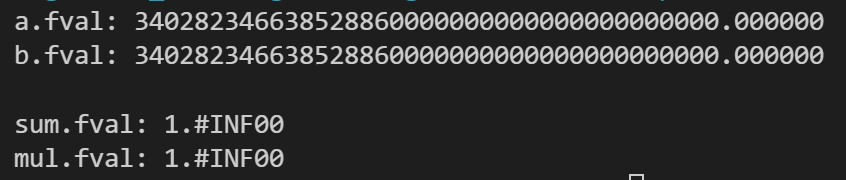
\includegraphics[width=0.8\textwidth]{assets/1.jpg}
\end{figure}

\paragraph{2)对应输入是规格化或非规格化数,而输出产生了阶码下溢结果为正(负)零的情况。}
加法时,只需要令两数为相反数即可。
\begin{lstlisting}[style=CStyle]
#include <stdio.h>
#include <stdlib.h>

void main(){
    union{
        unsigned int val;
        float fval;
    }a,b,sum, mul;

    a.val = 0x7f7fffff;
    b.val = 0xff7fffff;

    sum.fval = a.fval + b.fval;

    printf("a.fval: %f\n", a.fval);
    printf("b.fval: %f\n\n", b.fval);

    printf("sum.fval: %f\n", sum.fval);
    printf("sum.val: %08x\n", sum.val);
}
\end{lstlisting}

运行结果:
\begin{figure}[H]
    \centering
    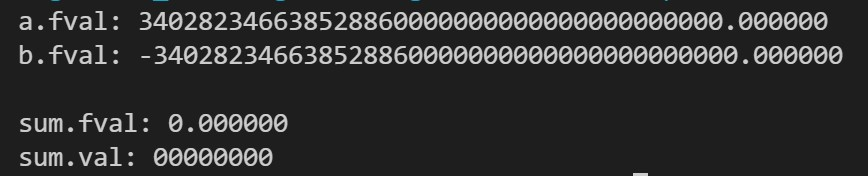
\includegraphics[width=0.8\textwidth]{assets/2.jpg}
\end{figure}

乘法时,令两数的阶码均极小,使得阶码下溢即可。
\begin{lstlisting}[style=CStyle]
#include <stdio.h>
#include <stdlib.h>

void main(){
    union{
        unsigned int val;
        float fval;
    }a,b,sum, mul;

    a.val = 0x80001;
    b.val = 0x80001;

    mul.fval = a.fval * b.fval;

    printf("a.fval: %e\n", a.fval);
    printf("b.fval: %e\n\n", b.fval);

    printf("mul.fval: %e\n", mul.fval);
    printf("mul.val: %08x\n", mul.val);
}
\end{lstlisting}

运行结果:
\begin{figure}[H]
    \centering
    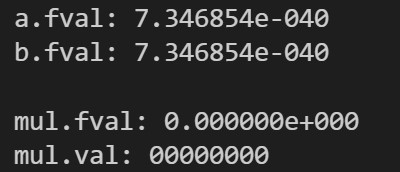
\includegraphics[width=0.5\textwidth]{assets/3.jpg}
\end{figure}

\section{心得体会}
\begin{enumerate}
    \item 指导手册与上课讲的内容对理解框架代码的实现原理很有帮助!很大程度上帮我克服了阅读理解源代码的恐惧感。
    \item 感觉参考资料稍微有点多,而且每个资料都只有含有部分信息?例如在guide里的对函数功能的注释不在源代码里,有些提示只在ppt里出现等等,找的时候稍微有点乱。
    \item 在写代码之前一定要先明确代码的功能是什么,有哪些情况,应该怎么实现,即先确保代码的正确性,然后再开始写。否则将在debug的过程中花费的精力远多于一开始提高代码的正确性所用的理论推导时间。例如在\verb|alu_sbb|函数的编写中就陷入了不停的debug写bug的过程,不如一开始就想好有哪些情况,怎样实现最简洁。
\end{enumerate}

\end{document}

% \begin{lstlisting}[style=CStyle]
% 
% \end{lstlisting}